%-------------------------------------------------------------------------------
% 请勿删除本注释
% Free Response Question 3
%
% 指引:
% 如在小问之前有通用问题描述,请放置于此
%-------------------------------------------------------------------------------
\begin{figure}[H]
\centering
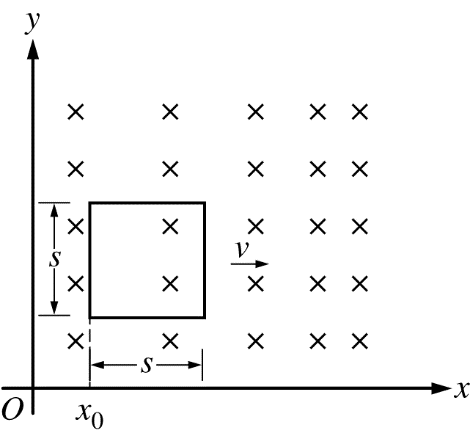
\includegraphics[scale=0.3]{images/img-021-029.png}
\end{figure}


\question
A square loop of conducting wire with resistance $R$ and with sides of length $s$ is located in the $x y$-plane. The loop is being pushed at constant speed $v$ by an external force of magnitude $F_{\text {ext }}$ in the $+x$-direction through a region with a magnetic field that is directed perpendicular to the $x y$-plane into the page, as shown in the figure above. The magnitude of the magnetic field as a function of position $x$ is given by the equation $B(x)=c x+B_{0}$, where $x$ is in meters, $c$ is a positive constant in $\mathrm{T} / \mathrm{m}$, and $B_{0}$ is a positive constant in teslas. The effects of gravity are negligible. % 请删除并替换本行,与上一行 \question 之间不要留空行

\begin{parts}

%-------------------------------------------------------------------------------
% 请勿删除本注释
% Part (a)
%
% 指引:
% 如在小问之前有通用问题描述,请放置于此
%-------------------------------------------------------------------------------

\part
Derive an expression for the magnetic flux through the loop when the left side of the loop is at position $x=x_{0}$. Express your answer in terms of $s, c, B_{0}, x_{0}$, and physical constants, as appropriate. % 请删除并替换本行,与上一行 \part 之间不要留空行

%-------------------------------------------------------------------------------
% 请勿删除本注释
% Part (b)
%
% 指引:
% 如在小问之前有通用问题描述,请放置于此
%-------------------------------------------------------------------------------

\part
Derive an expression for the magnitude of the induced current in the loop, if any. Express your answer in terms of $R, s, v, c, B_{0}, x$, and physical constants, as appropriate.  % 请删除并替换本行,与上一行 \part 之间不要留空行

%-------------------------------------------------------------------------------
% 请勿删除本注释
% Part (c)
%
% 指引:
% 如在小问之前有通用问题描述,请放置于此
%-------------------------------------------------------------------------------

\part
Is the induced current in the loop clockwise, counterclockwise, or zero?

\underline{\qquad}Clockwise \qquad \underline{\qquad}Counterclockwise \qquad \underline{\qquad}Zero

Justify your answer. % 请删除并替换本行,与上一行 \part 之间不要留空行

%-------------------------------------------------------------------------------
% 请勿删除本注释
% Part (d)
%
% 指引:
% 如在小问之前有通用问题描述,请放置于此
%-------------------------------------------------------------------------------

\part
When the left side of the loop is at position $x=x_{0}$ and moving with constant speed $v$, what is the direction of the net magnetic force, if any, on the loop? % 请删除并替换本行,与上一行 \part 之间不要留空行

\underline{\qquad}Toward the top of the page  \underline{\qquad}Out of the page \underline{\qquad}Left

\underline{\qquad}Toward the bottom of the page  \underline{\qquad}Into the page \underline{\qquad}Right

\underline{\qquad}Undefined, because the net magnetic force on the loop is zero.

Justify your answer.

%-------------------------------------------------------------------------------
% 请勿删除本注释
% Part (e)
%
% 指引:
% 如在小问之前有通用问题描述,请放置于此
%-------------------------------------------------------------------------------

\part
Derive an expression for the magnitude of the external force $F_{e x t}$ exerted on the loop to keep it moving at a constant speed when the loop is at position $x=x_{0}$. Express your answer in terms of $R, s, v, c, B_{0}, x_{0}$, and physical constants, as appropriate. % 请删除并替换本行,与上一行 \part 之间不要留空行

%-------------------------------------------------------------------------------
% 请勿删除本注释
% Part (f)
%
% 指引:
% 如在小问之前有通用问题描述,请放置于此
%-------------------------------------------------------------------------------

\part
Rank, with 1 being the largest, the magnitude of the magnetic force on the four sides of the loop. If two sides have the same magnetic force, give them the same numerical ranking. % 请删除并替换本行,与上一行 \part 之间不要留空行

\underline{\qquad}Left  \qquad \underline{\qquad}Right \qquad \underline{\qquad}Top \qquad \underline{\qquad}Bottom

\end{parts}
